\documentclass[11pt,leqno]{article}
\usepackage[spanish,activeacute]{babel}
\usepackage[utf8]{inputenc}
\usepackage{enumerate}
\usepackage{float}
\usepackage{pdfpages}
\usepackage[hidelinks]{hyperref}
\usepackage{booktabs} 
\usepackage{eurosym}


\author{Jacinto Carrasco Castillo \\
		\href{jacintocc@correo.ugr.es}{jacintocc@correo.ugr.es}}
		
\title{Emprendimiento y transferencia del conocimiento.\\ Trabajo práctico}

\makeindex

\begin{document}

\maketitle
\tableofcontents

\newpage

\section*{Introducción - VennChat}
\label{sec:intro}
\addcontentsline{toc}{section}{\nameref{sec:intro}}

	Antes de comenzar el desarrollo del modelo de negocio vamos a exponer la
	idea general del producto. 
	El principal motivo de la propuesta reside en que, en la
	actualidad, las aplicaciones de mensajería instantánea
	se vuelven inmanejables o incluso molestas, 
	debido a la proliferación de grupos o canales, de los que muchos comparten
	el mismo propósito y cuya diferencia se encuentra en una pequeña 
	parte de los componentes. Además, es habitual que en los grupos se mezclen 
	conversaciones de trabajo con asuntos ajenos a éste, 
	con lo que no resulta efectivo silenciar ciertas conversaciones; 
	que ciertos grupos cambien de nombre o imágen y se confundan destinatarios
	o que el mismo mensaje
	de la misma persona llegue por vías distintas.\\
	La idea es, en primer lugar, 
	que los grupos no sean estructuras fijas e independientes,
	sino poder navegar entre ellas como si de un gran diagrama de Venn se
	tratase, 
	con subgrupos contenidos en otros para hablar de temas más específicos 
	y la posibilidad de modificar el grupo al que se le pretende
	mandar cada mensaje. 
	También se propone para empresas la posibilidad de que los usuarios 
	dispongan de varios perfiles, con lo que se dispondría de un filtro rápido
	para notificaciones y conversaciones. 
	Por último, se propone la integración de otras 
	herramientas y aplicaciones de productividad como la realización
	de listas, votaciones y elección de fechas o gestión de proyectos
	mediante tableros.\\
	Una idea similar aunque enfocada en otro aspecto, fue la llevada
	a cabo en Google+, plataforma que no ha obtenido el éxito esperado, sin
	embargo en el contexto de una red social se tiende a tener menos grupos
	de personas con los que compartir contenidos y la clasificación
	se realiza por niveles: mejores amigos, amigos, familiares y conocidos.
	Esta funcionalidad ya se incluyó en el principal competidor como
	red social, Facebook, con lo que las posibles ventajas de Google+ han
	quedado poco claras. Sin embargo, en la aplicación descrita
	sí se presentan ventajas claras con respecto a la competencia enfocadas
	en la mejora de la productividad de los equipos.

\section{Modelo de negocio: CANVAS - DAFO - Análisis de debilidades y fortalezas}


\subsection{Modelo CANVAS}

\noindent\makebox[\textwidth]{
	\includegraphics[width=1.6\textwidth]{CANVAS.pdf}
 	\label{fig:CANVAS}
}

\newpage
\subsection{Análisis DAFO}
\label{ssec:DAFO}

\subsubsection{Análisis interno}

\paragraph{Debilidades}
\begin{description}
	\item[Novedad] Empresa nueva en un sector copado por aplicaciones ya asentadas. 
	Dificultad para sustituir a estas aplicaciones en el público general pues se 
	han convertido en formas de comunicación estándar, como lo fueron el teléfono
	o el SMS.
	\item[Fondos] Fondos disponibles actualmente muy
	limitados. 
	\item[Inexperiencia]	Nula experiencia empresarial. 
	\item[Márqueting] Poca experiencia en márqueting. 
	\item[Diseño] La idea es fuertemente dependiente de que el diseño sea a
	la vez atractivo y lo suficientemente sencillo como para que las operaciones
	que deseamos llevar a cabo sean muy intuitivas. La experiencia
	del equipo se ciñe al terreno del desarrollo de aplicaciones, 
	falta de experto en diseño.
	\item[Idiomas] Escaso conocimiento de idiomas más allá de español e
	inglés.
	\item[Problema de escalabilidad] Actualmente se cuenta únicamente con una pequeña
	granja de servidores.
\end{description}	

\paragraph{Fortalezas}
\begin{description}
	\item[Novedad] Nuevo control de grupos diferente al de las aplicaciones 
	existentes, más dinámico y visual. Esto permite un mejor control sobre las 
	conversaciones, no dependiente de los correspondientes administradores
	de grupos.
	\item[Integración] Posibilidad de incluir aplicaciones externas tales como
	calendarios o \textit{boards} para la organización de equipos.
	\item[Perfiles] Separación mediante perfiles de las conversaciones
	del ámbito personal al profesional, 
	lo que hace a la aplicación especialmente atractiva para la empresa.
	\item[Desarrolladores] El equipo está formado por expertos desarrolladores
	de aplicaciones. 
	\item[Seguridad] Contamos en la empresa con un estudiante de doctorado
	que está desarrollando su tesis en el ámbito de la seguridad en las 
	comunicaciones.
\end{description}	
	
\subsubsection{Análisis externo}
	
\paragraph{Amenazas}

\begin{description}
	 \item[Aplicaciones existentes] Empresas en el sector ya consolidadas, 
	 orientadas a comunicación con pequeños grupos. Podrían desarrollar nueva 
	 funcionalidad orientada al manejo de grupos de trabajo, aunque su trayectoria
	 indica que se centran en ofrecer más funcionalidades para usuarios
	 no profesionales. 

	 \item[Rigidez de empresas] Reticencia por parte de las empresas a cambiar
	 sus sistemas propios de comunicación. 

\end{description}
	
\paragraph{Oportunidades}
\begin{description}

	\item[Público abierto] Pensado para profesionales tecnológicos, usualmente 
	abiertos a probar diferentes aplicaciones y quedarse con la 
	que ofrezca.
	\item[Más involucrados] Conforme pasa el tiempo los usuarios son más 
	expertos y quieren tener
	un mayor control sobre la organización de las conversaciones. Esta aplicación
	ofrece este control al usuario, creando perfiles para separar conversaciones.
	\item[Codigo abierto] Cada vez más personas están interesadas en soluciones
	de código abierto a la que se le puedan integrar pequeños programas o 
	complementos con los que cada usuario o empresa pueda personalizar detalles
	de la aplicación. Se puede incluir un sistema de recompensas, por ejemplo 
	ofreciendo la funcionalidad \textit{premium}, para aquellos desarrolladores
	cuyas mejoras sean positivamente valoradas por la comunidad.
\end{description}


\subsubsection{Propuestas para solucionar debilidades y amenazas}

\begin{description}
	\item[Fondos] Se pretende acudir a rondas de financiación para incrementar
	los fondos disponibles para la empresa.
	
	\item[Inexperiencia empresarial] Actualmente uno de los componentes del
	equipo está realizando un máster MBA. Además, aunque no es la única acción
	que se está realizando en ese sentido, se tiene previsto acudir a un 
	programa de mentorización para pequeñas empresas promovido por La Caixa.
	
	\item[Equipo] Para solucionar los problemas de la falta de personal se pretende
	contratar inicialmente a dos diseñadores y a un traductor para aumentar los 
	idiomas disponibles en la aplicación. En un primer momento se puede 
	externalizar la traducción de la aplicación pagando por ella como
	proyecto. 
	
	\item[Publicidad] Para obtener publicidad al inicio se ha contactado con 
	revistas y blogs de tecnología para que realicen una crítica de la
	aplicación.
	
	\item[Servidores disponibles] Con el objetivo de tener una mayor disponibilidad
	y de poder soportar la carga de un mayor número de usuarios se prevee
	aumentar el número de servidores.
	
\end{description}
	 
	 
	 
	 
	 
	 
	 
	 
	 
	 
	 
	 
	 
	 
	 
	 
	 
	 
	 
\newpage
\section{Ficha de búsqueda de financiación empresarial}

\begin{enumerate}
\item  Datos administrativos

	\begin{enumerate}[a]
\item Nombre de la empresa: Diagram Communications. 
\item Nombre del proyecto: VennChat.
\item Breve descripción del proyecto:  Aplicación de mensajería instantánea
con una gestión más fluida de las conversaciones. Los grupos se tratan como 
conjuntos a los que aplicar las operaciones habituales: intersección, unión y
diferencia.

	\end{enumerate}

\item Equipo

\begin{enumerate}[a]
\item Miembro principal del equipo: Graduado en Informática y Matemáticas. Promotor de la idea y principal desarrollador.
\item Otros miembros del equipo: 
	\begin{itemize}
	\item Ingeniera informática experta en gestión de sistemas. 
	\item Ingeniero en telecomunicaciones.
	 Doctorando en protocolos de encriptación.
	\item Ingeniero informático. Actualmente realizando un máster MBA.
	\item Ingeniero informático y desarrollador de aplicaciones.	
	\end{itemize}

\item Papeles cubiertos por el equipo 

	Los papeles cubiertos son los de desarrolladores y técnicos.
	El miembro que está realizando actualmente un máster MBA será
	quien se encargue de las labores de gestión de la empresa, la 
	gestión comercial y el \textit{marketing}. 
	
\item Experiencia emprendedora previa (años de experiencia, iniciativas, etc):

	No se cuenta con experiencia previa en el terreno de la creación 
	de empresas, sin embargo este mismo equipo ha participado en
	concursos de proyectos de software libre o retos 
	tecnológicos.
	
\item Necesidades del equipo 

	Como se ha comentado en el análisis DAFO (\ref{ssec:DAFO}), 
	la necesidad más urgente es la de al menos dos diseñadores para
	la aplicación móvil y la aplicación de escritorio. 
	También será necesario la contratación de al menos un traductor en
	un primer momento para que la aplicación esté disponible para los 
	idiomas con más potenciales usuarios.
	
\item Otros compromisos del equipo de emprendedores

	Como se ha comentado, actualmente hay un miembro que está realizando
	un máster y otro que está finalizando su doctorado, con lo que la
	dedicación a la empresa es reducida.
	
\end{enumerate}


\item Oportunidad de negocio

\begin{enumerate}[a]
\item Problema / Necesidad 

	En la actualidad, las aplicaciones de mensajería instantánea, 
	por el excesivo uso de ellas, se han vuelto incluso molestas, 
	en especial cuando también se usan para la comunicación de equipos
	de trabajo.

\item Producto / Servicio 

	El producto ofrecido es una aplicación de mensajería instantánea
	orientada a la comunicación entre grupos de trabajo, en el que 
	las conversaciones se identifican como el conjunto de participantes 
	que están en la conversación.

\item  Mercado objetivo 

	El mercado objetivo está en los usuarios de aplicaciones 
	de mensajería instantánea que requieren también de un canal 
	de comunicación rápida en su trabajo.	Especialmente estas personas 
	habrán encontrado incómodo, improductivo y estresante el 
	uso de estas aplicaciones, con lo que buscamos presentarle una aplicación
	que le facilite el control sobre sus comunicaciones.
	
\item Competencia 

	La competencia no ha centrado su producto en estos usuarios 
	activos e informados sino en el público general, con lo que
	se pensarán un cambio en la gestión tradicional de las conversaciones.
	
	
\item Estrategia de adquisición de clientes

	Para la captación de clientes se pretende realizar en un primer momento
	un gran esfuerzo en publicidad para llegar a usuarios y empresas que,
	recordemos, serán las que hagan aportaciones económicas. Es importante
	que el producto esté terminado para que la aplicación no sea 
	desechada por quien la pruebe.
	
\item Análisis de Riesgos

	Los principales riesgos son que la aplicación no resulte lo suficientemente
	atractiva para los usuarios, amenaza que pretendemos minimizar
	con el estudio previo al lanzamiento de la empresa; y la copia 
	por parte de los competidores, cuestión que se considera poco probable
	por las cuestiones comentadas previamente.	
	
\item Estado de desarrollo y hoja de ruta hasta el producto/servicio final.

	De la aplicación se tiene un prototipo básico. Aunque está implementada
	la funcionalidad descrita para las conversaciones, es necesario aún
	crear la interfaz que haga que sea natural. Esta fase se espera 
	alcanzar a principios de otoño de este año y a finales de año
	se espera disponer del producto final con la posibilidadad de incluir
	herramientas externas.
\end{enumerate}




\item Tecnología

\begin{enumerate}[a]
\item Descripción de la tecnología

	Novedosa aplicación de mensajería enfocada para grupos de trabajo
	y una mayor funcionalidad para el manejo de las conversaciones.
	
\item Innovación tecnológica

	Diferenciación con respecto a las demás aplicaciones de mensajería
	el manejo de las conversaciones y el enfoque en la productividad.
	
\item Propiedad Intelectual. Libertad para actuar. 
Barreras de conocimiento frente a competidores.

	En principio la barrera de conocimiento frente a competidor es 
	baja pues consiste únicamente en el desarrollo de la aplicación.
	
\end{enumerate}



\item Finanzas

\begin{enumerate}[a]
\item  Modelo de coste/beneficio

	Según las cuentas disponibles en el cuadro \ref{PyG}, obtenemos un
	modelo coste/beneficio
	\[ \frac{B}{C} = 1.35 	\]
	
\item  Necesidades de financiación 
	
	Puesto que estamos en la primera fase del negocio, necesitamos un gran impulso
	económico inicial estimado en 100000\euro, para garantizar la solvencia de la 
	empresa en los momentos iniciales, pudiendo recuperar esta inversión en el 
	transcurso del tercer año.
	
\end{enumerate}



\item Caracterización de la propuesta 
(escoger una de las opciones o dar un valor numérico)

\begin{enumerate}[a]
\item Originalidad

	Uno de los elementos fundamentales de la propuesta es la originalidad y
	la diferenciación con respecto a las alternativas existentes.
\item  Grado de madurez de la propuesta

	Como se ha descrito, se ha desarrollado ya un prototipo de
	la propuesta. 
\item Posición de la cadena de valor 

	Seremos los desarrolladores de la idea.
\item Origen de la idea de innovación 

	El origen de la idea es la necesidad personal de una aplicación de este
	tipo.
	
\item  Años de experiencia en gestión

	No se tiene experiencia en la gestión de una empresa.
\item Años de experiencia en tecnología

	Todos los integrantes han estudiado en el ámbito tecnológico
	y han trabajado al menos un año en empresas del sector.
\item Sector de mercado principal 
	
	Telecomunicaciones.
\item Tipo de mercado 
	
	Los clientes serán principalmente empresas que deseen usar la aplicación
	como canal de comunicación entre los empleados.
\item Marco geográfico 

	Global.
\item  Grado de realización de la tecnología: 3
\item Grado de maduración del modelo de negocio: 1

\item Potencial beneficio por parte del usuario 

	Mejora con respecto a las aplicaciones actuales.
\end{enumerate}


\end{enumerate}

	
	
\section{Ejercicio práctico de búsqueda de patentes}

\subsection{Ejercicio 1}
Buscar Patentes de relacionadas con el campo de vuestra idea de negocio 
(por ejemplo patentes relacionadas con redes neuronales, patentes relacionadas 
con lógica difusa, etc. si vuestra idea de negocio o tecnología se relaciona con ``soft-computing"). 
Buscar con palabras clave (key words).

\paragraph{Transmission Security Protocol}
\begin{enumerate}[a]
\item ¿Cuántas son? 

	475000 patentes
\item Indicar las tres principales empresas que tiene patentes en este campo.

	IBM, Microsoft y Qualcomm.
\item Buscar una patente en concreto e indicar el link donde aparezcan los 
\textit{claims} de una patente en este campo.

	\url{https://www.lens.org/lens/patent/US_2015_0350246_A1}
\end{enumerate}


\paragraph{XMPP}
\begin{enumerate}[a]
\item ¿Cuántas son? 

	9200 patentes
\item Indicar las tres principales empresas que tiene patentes en este campo.

	Apple, Google y Seven Networks Inc.
\item Buscar una patente en concreto e indicar el link donde aparezcan los 
\textit{claims} de una patente en este campo.

	\url{https://www.lens.org/lens/patent/US_9503529_B2}
\end{enumerate}


\subsection{Ejercicio 2}
Buscar patentes de una empresa en el campo en el que se desarrolla 
vuestra idea de negocio.
Indicar brevemente (como máximo en una media página), cuántas son y 
fundamentalmente en qué temáticas (sólo indicar los dos campos principales en 
los que existan patentes).
Sugerencia: utilizar lens.org para ver la CIP (o ICP o IPCR) de las patentes y 
filtrar usando sólo
los cuatro primeros 4 dígitos. Utilizar también truncamientos para el nombre de 
la empresa.

Describiremos las patentes realizadas por Whatsapp Inc.:
\begin{itemize}
\item Tiene 45 patentes.
\item La mayoría de patentes realizadas tienen que ver con la identificación
de teléfonos y número de teléfonos; el control de contenidos para 
evitar \textit{spam} teniendo en cuenta el número de usuarios que han 
bloqueado previamente el número o el ratio de mensajes enviados y recibidos;
llamadas VOIP o gestión dinámica del contenido multimedia.
\end{itemize}

\subsection{Ejercicio 3}
A la hora de valorar patentes se puede tener en cuenta el crecimiento del área 
tecnológica, que a su vez se puede medir de forma indirecta analizando el 
crecimiento registrado en el número de solicitudes de patente en un área 
específica de la tecnología, valorando
positivamente aquellas tecnologías cuyas patentes hayan registrado un 
crecimiento continuado en el pasado reciente (20 años) frente a las que hayan 
registrado un crecimiento negativo, discontinuo o alejado en el tiempo.
Buscar tendencias de patentes en las siguientes temáticas (utilizar el buscador ``lens").
Para cada caso añadir el gráfico de tendencia anual de patentes sobre esta temática:
\begin{enumerate}
\item Buscar patentes sobre ``Face recognition". Indicar cuántas 
tiene ``Samsung" sobre esta temática.

Samsung tiene 2863 patentes en este campo.

\begin{figure}[h!]
\centering
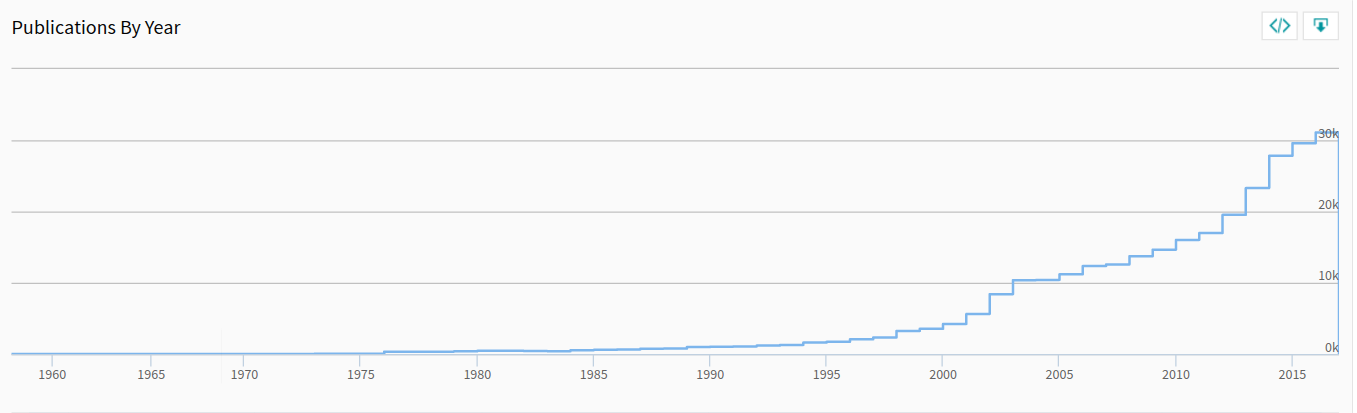
\includegraphics[width=0.8\textwidth]{Face}
\caption{Evolución de las patentes realizadas sobre reconocimiento facial}
\end{figure}

\item Buscar patentes sobre ``Fuzzy logic". 
Indicar cuántas tiene ``Microsoft" sobre esta temática.

Microsoft tiene 8400 patentes sobre esta temática.

\begin{figure}[h!]
\centering
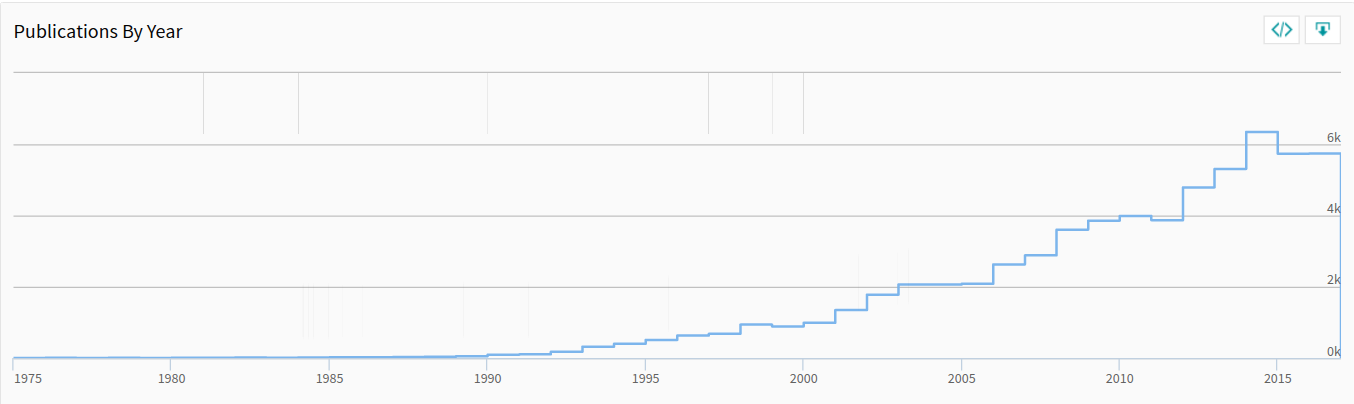
\includegraphics[width=0.8\textwidth]{Fuzzy}
\caption{Evolución de las patentes realizadas sobre lógica difusa}
\end{figure}
\item Buscar patentes sobre ``SVM" (Support Vector Machine). 
Indicar cuántas tiene ``Microsoft" sobre esta temática.

Microsoft tiene 12800 patentes sobre esta temática.

\begin{figure}[h!]
\centering
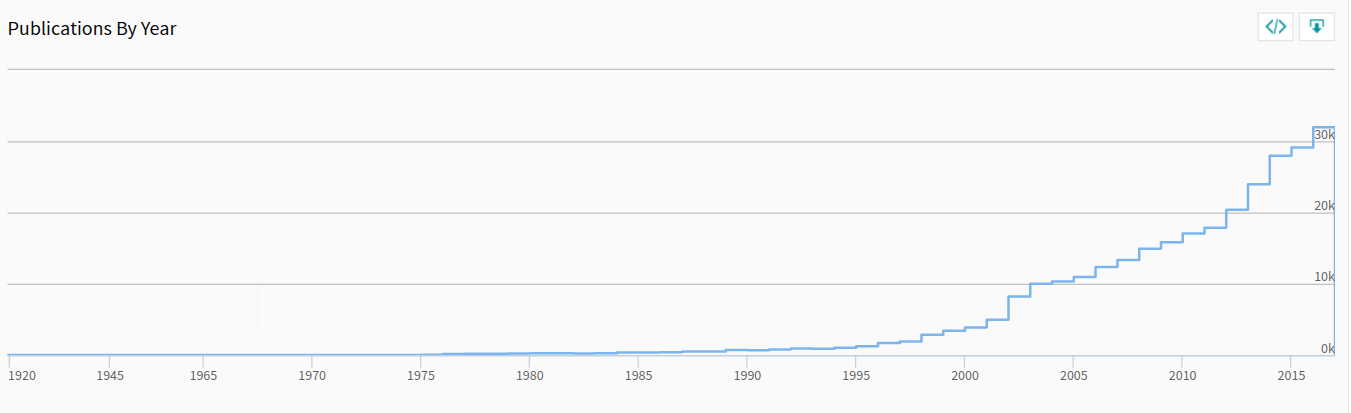
\includegraphics[width=0.8\textwidth]{SVM}
\caption{Evolución de las patentes realizadas sobre SVM}
\end{figure}
\end{enumerate}

















\newpage
\section{\textit{Elevator Pitch}}

	El vídeo con el \textit{elevator pitch } se encuentra en \url{https://youtu.be/MYr6Gk-Z9H}.
	
\section{Tabla con previsiones financieras}

% Please add the following required packages to your document preamble:
% \usepackage{booktabs}
\begin{table}[H]
\centering
\caption{Balance general}
\label{BG}% Please add the following required packages to your document preamble:
\begin{tabular}{@{}lllll@{}}
\toprule
                           &                                   & 2017   & 2018   & 2019   \\ \midrule
Activos                    &                                   &        &        &        \\ \midrule
                           & Cuenta Corriente                  & 100000 & 75000  & 83000  \\
                           & Clientes                          & 0      & 20500  & 40000  \\
                           &                                   &        &        &        \\
Activo Corriente           &                                   & 100000 & 95500  & 123000 \\ \midrule
                           & Equipos personales                & 4550   & 5700   & 6000   \\
                           & Servidores                        & 6000   & 15000  & 20000  \\
                           & Mobiliario                        & 850    & 950    & 1300   \\
                           &                                   &        &        &        \\
Propiedad, planta y equipo &                                   & 111400 & 117150 & 150300 \\ \midrule
Activo Total               &                                   & 211400 & 212650 & 273300 \\ \midrule
Pasivo                     &                                   &        &        &        \\ \midrule
                           & Obligaciones laborales            & 10000  & 0      & 0      \\
                           & Impuestos                         & 1500   & 7500   & 13500  \\
                           & Préstamos a corto plazo           & 2000   & 5000   & 7000   \\
                           &                                   &        &        &        \\
Pasivo corriente           &                                   & 13500  & 12500  & 20500  \\ \midrule
                           & Préstamos bancarios a largo plazo & 20000  & 13000  & 6000   \\
                           &                                   &        &        &        \\
Deuda a largo plazo        &                                   & 20000  & 13000  & 6000   \\ \midrule
Pasivo Total               &                                   & 33500  & 25500  & 26500  \\ \midrule
                           & Patrimonio                        & 177900 & 180400 & 223700 \\
                           & Reserva                           &        & 6750   & 23100  \\
                           &                                   &        &        &        \\
Total patrimonio           &                                   & 177900 & 187150 & 246800 \\ \midrule
Total pasivo y patrimonio  &                                   & 211400 & 212650 & 273300 \\ \bottomrule
\end{tabular}
\end{table}



\subsection{Tabla de pérdidas y ganancias}

% Please add the following required packages to your document preamble:
% \usepackage{booktabs}
\begin{table}[H]
\centering
\caption{Tabla de pérdidas y ganancias}
\label{PyG}
\begin{tabular}{@{}lllll@{}}
\toprule
                    &                                     & 2017   & 2018   & 2019   \\ \midrule
Ingresos            &                                     &        &        &        \\
                    & Venta de la aplicación              & 0      & 102560 & 249340 \\
                    & Venta de publicidad                 & 0      & 57400  & 103260 \\
                    & Trabajos realizados (I+D)           & 95700  & 110000 & 105000 \\
                    &                                     &        &        &        \\
                    & Total ingresos                      & 95700  & 269960 & 457600 \\
                    &                                     &        &        &        \\
                    &                                     &        &        &        \\
Gastos              &                                     &        &        &        \\
                    &                                     &        &        &        \\
                    & Gastos personal                     & 116400 & 128400 & 130000 \\
                    & Aprovisionamientos                  & 21400  & 36000  & 40000  \\
                    & Trabajos externalizados             & 12000  & 7000   & 8000   \\
                    & Impuestos indirectos a la actividad & 1500   & 2000   & 2000   \\
                    & Gastos de explotación               & 22000  & 39000  & 45000  \\
                    & Enajenaciones del inmovilizado      &        & 700    & 1200   \\
                    &                                     &        &        &        \\
                    &                                     &        &        &        \\
                    & Total gastos                        & 173300 & 213100 & 226200 \\
                    &                                     &        &        &        \\
BAII                &                                     & -77600 & 56860  & 231400 \\
BAI                 &                                     & -77600 & 56860  & 231400 \\
Resultado ejercicio &                                     & -82385 & 11370  & 138000 \\ \bottomrule
\end{tabular}
\end{table}


\subsection{Estado de la tesorería}

% Please add the following required packages to your document preamble:
% \usepackage{booktabs}
\begin{table}[H]
\centering
\caption{Estado de la tesorería}
\label{tesoreria}
\begin{tabular}{@{}lllll@{}}
                                    &        & 2017   & 2018   & 2019   \\
SALDO INICIAL                       & 100000 & 100000 & 5700   & 1760   \\
                                    &        &        &        &        \\
Pagos                               &        &        &        &        \\
Gastos personal                     &        & 106400 & 133400 & 140000 \\
Aprovisionamientos                  &        & 15400  & 8500   & 35000  \\
Trabajos externalizados             &        & 6000   & 1000   & 19000  \\
Impuestos indirectos a la actividad &        & 1500   & 2000   & 2000   \\
Gastos de explotación               &        & 13000  & 39000  & 45000  \\
Préstamos a corto plazo             &        & 2000   & 5000   & 7000   \\
                                    &        &        &        &        \\
Total gastos                        &        & 144300 & 188900 & 248000 \\
Ingresos                            &        &        &        &        \\
                                    &        &        &        &        \\
Venta de la aplicación              &        & 0      & 122560 & 249340 \\
Venta de publicidad                 &        & 0      & 57400  & 103260 \\
Aportaciones al capital             &        & 50000  & 5000   & 0      \\
                                    &        &        &        &        \\
Total ingresos                      &        & 50000  & 184960 & 352600 \\
SALDO FINAL                         &        & 5700   & 1760   & 106360
\end{tabular}
\end{table}








\newpage
\section{Desarrollo de creatividad y liderazgo}
\subsection{Binomio fantástico}	

\paragraph{Wooded Question}

	\textit{(Las palabras, que debíamos seleccionar aleatoriamente,
	se han obtenido por ser el primer adjetivo y sustantivo de las
	definiciones de dos entradas de una lista de correo de palabras en inglés.)}\\
	Ante un problema cada vez más patente como es el cambio climático, la sociedad
cada vez se interesa más en la huella ecológica de sus actos.
La aplicación \textbf{Wooded Question} nos responde a esta pregunta a la vez que 
le va dando una nueva dimensión. La aplicación, como propósito general,
calcula la emisión de CO$_2$ producida por nuestra actividad y además 
el número de árboles que serían necesarios para contrarrestar esta emisión.
Sin embargo, y es por esto por lo que se comentaba que le daba una nueva dimensión
a la pregunta, gracias a la aplicación se podrá transmitir cierta información 
de la que muchas veces no se dispone como por ejemplo del enorme gasto 
que supone en combustible el consumo de ciertos productos importados o
el embalaje, en comparación con cuestiones sobre las que estamos más concienciados
como el transporte que utilizamos para desplazarnos a nuestro centro de
trabajo o el gasto en calefacción o aire acondicionado.\\
Para motivar el uso de la aplicación y no ser simplemente una conciencia 
que advierte al usuario de que está contaminando, también se mostrará la 
cantidad de gases que estamos dejando de emitir con un (esperable) cambio
de hábitos de consumo conforme vamos haciéndonos conscientes. También 
se propone incluir en la aplicación un sistema para realizar 
donaciones a asociaciones que se dediquen a la plantación de árboles 
o asociaciones ecologistas.\\
Para llevar a cabo esta idea podríamos presentarla incluso a las asociaciones
mencionadas para que fueran quienes costeasen la producción de la aplicación.



\newpage
\subsection{Ejercicio de liderazgo}

\textit{Describa una situación personal/laboral de liderazgo
(haya sido líder o le hayan liderado) en la que haya visto
la necesidad (o no) de aplicar distintas estrategias de
liderar.}


	Una situación habitual en la que es muy palpable la necesidad de diferentes
tipos de liderazgo se producen en los habituales y cada vez más frecuentes
\textit{hackatones} y eventos similares. En muchos de ellos los participantes
comienzan un proyecto que se pretende terminar en un corto período de tiempo 
o se adhieren a uno ya iniciado para ayudar al creador a completarlo.
Como experiencia personal, he participado en alguno de los organizados por la
Oficina del Software Libre en relación al Certamen de Proyectos Libres. En este 
tipo de eventos, las habilidades de los participantes son dispares y el líder
(quien haya presentado el proyecto), no sólo debe aplicar una técnica de liderazgo 
distinta según la persona, sino también según el momento.

\begin{enumerate}
\item Al principio del \textit{hackaton}, el liderazgo debe ser de tipo directivo,
pues los objetivos del proyecto son únicamente conocidos por el líder. Además,
debe conocer las habilidades de cada voluntario, con lo que 
al principio deberá estar más encima de aquellos que sean novatos en el tema
para que tengan claro qué tienen que hacer.
\item Por la naturaleza de la tarea, el liderazgo pasará rápidamente a ser de tipo
persuasivo, pues al no haber normalmente una retribución económica por el 
desarrollo del trabajo, los participantes deben sentirse cómodos, deben 
saber por qué están haciendo lo que están haciendo y deben sentirse escuchados.
\item Conforme avanza el \textit{hackaton} lo habitual será que los participantes ya
tengan ideas propias sobre posibles mejoras para el proyecto en el que
decidieron participar. El líder deberá escucharlos y seguramente el proyecto
gane con la inclusión de algunas de estas propuestas.
\item A la etapa delegativa no se suele llegar en este tipo de eventos, 
ya que el tiempo es muy reducido y el líder podrá delegar tareas menores 
pero deberá siempre estar siguiendo el estado del proyecto, participando
en el desarrollo también de éste.
\end{enumerate}


\end{document}